\section{Разработка корпуса}
\label{sec:case}

\subsection{Выбор материала и метода изготовления корпуса}

Для создания корпуса устройства была выбрана 3D-печать с помощью PET-G пластика. Этот выбор обусловлен несколькими причинами:

\begin{enumerate}
    \item PET-G пластик обладает высокой механической прочностью, 
    что обеспечивает нужную жесткость и точность всех компонентов устройства.
    \item PET-G легко поддается обработке, что упрощает процесс 3D печати. 
    А небольшая температура плавления позволяет корректировать устройство по мере его сборки.
    \item Этот пластик широко доступен и относительно недорог, из-за чего он экономически выгоден для 
    прототипирования и мелкосерийного производства.
    \item Метод 3D печати позволяет быстро и легко вносить изменения в конструкцию корпуса, 
    что особенно важно на этапе разработки и тестирования устройства.
\end{enumerate}

Таким образом, PET-G пластик обеспечивает оптимальное сочетание прочности, устойчивости, экономичности и гибкости в дизайне.

\subsection{Проектирование корпуса}

Как упоминалось ранее, суть гравировки заключается в поэтапном движении двух частей устройства: платформы
с заготовкой (Ось Y) и лазера (Ось X). Чтобы заготовка не соскальзывала с платформы она фиксируется 8 магнитами 
с внешней и с обратной стороны платформы. Для правильного и точного движения платформы и лазера необходимо по две 
направляющих на каждый движущийся модуль. Для данной цели выбраны металлические направляющие DVD-привода, 
по которым выезжает отсек для DVD-диска. 

\begin{figure}[ht]
    \centering
    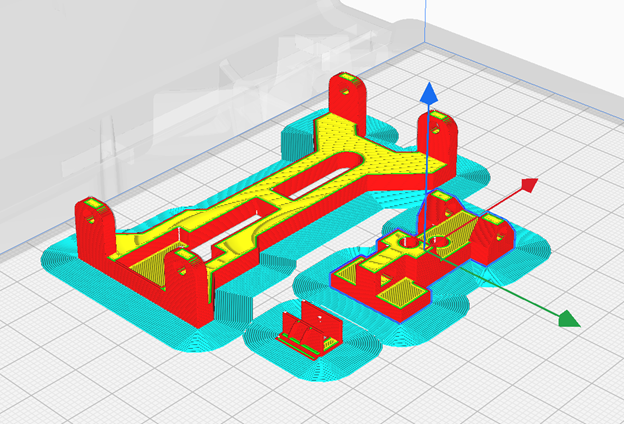
\includegraphics[width=0.5\linewidth]{\commonSecPathPrefix/sec_6/content/slider.png}
    \caption{Слайдер, зажим и посадочное место для двигателя}
    \label{fig:slider}
\end{figure}


Так как направляющим соответственно передвигается сама платформа и держатель лазера, то необходимо обеспечить правильный 
механизм передачи движения от мотора к модулям. Для этого сделаны специальные держатели  
для фиксации модулей на направляющих и небольшие зажимы (рис. \ref{fig:slider}), которые соединяют резьбу шагового двигателя и держатели модулей. 

Чтобы зафиксировать лазер, двигатель и пластиковые передвигающиеся по Оси X модули были сделаны две стойки, 
между которыми и закрепляется данная конструкция. 

В качестве крепления для мотора Оси Y и стоек спроектировано прямоугольное основание, показанное на рисунке \ref{fig:base},
с выемкой для мотора и платформы.

\begin{figure}[ht]
    \centering
    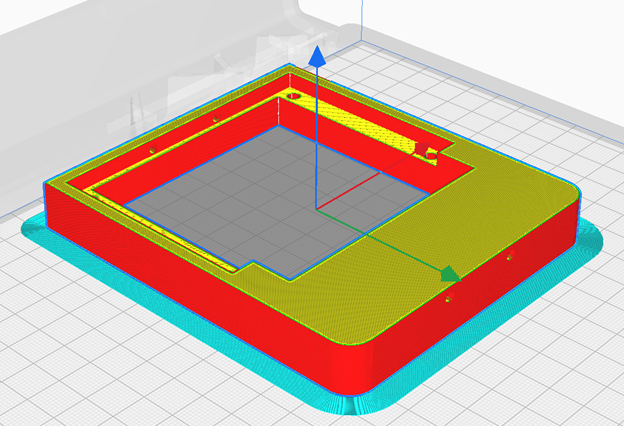
\includegraphics[width=0.5\linewidth]{\commonSecPathPrefix/sec_6/content/base.png}
    \caption{Основание устройства}
    \label{fig:base}
\end{figure}

Для платы предусмотрено отдельное крепление за модулем лазера и его шаговым мотором.

Суммарные затраты пластика составили 126 грамм, а время печати порядка 7,5 часов (рис. \ref{fig:frame}).

\begin{figure}[ht]
    \centering
    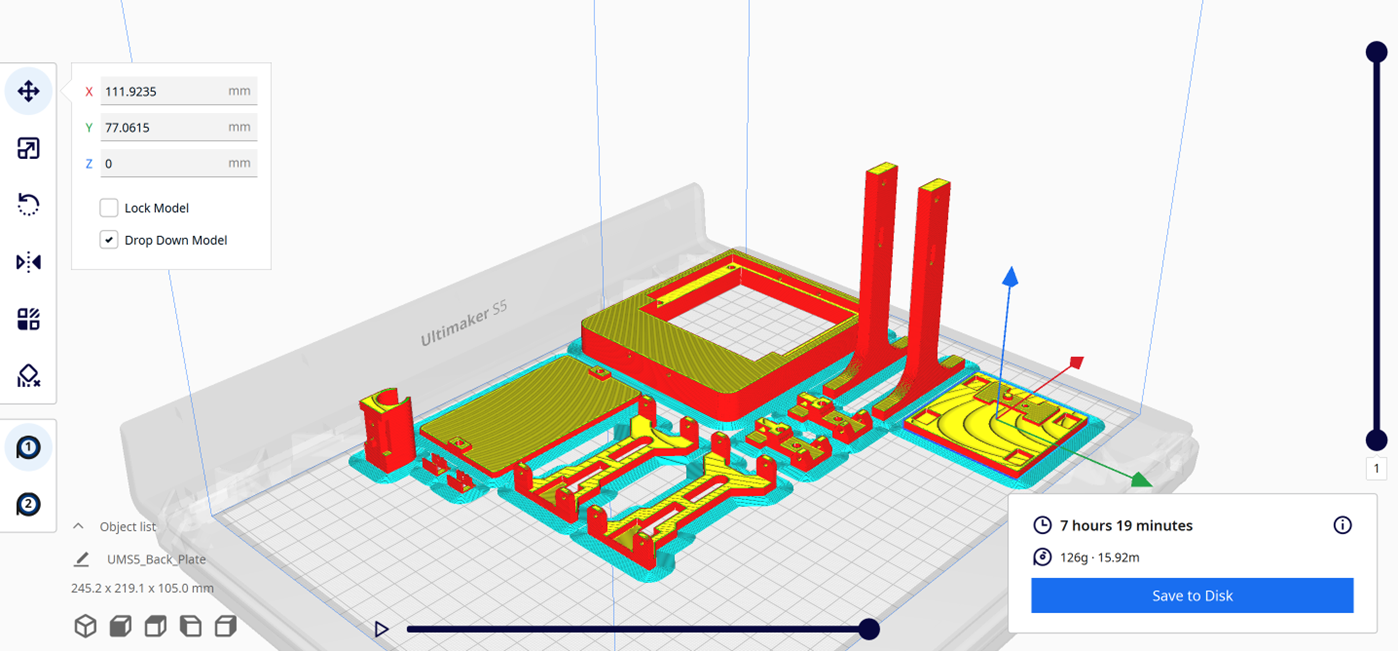
\includegraphics[width=0.9\linewidth]{\commonSecPathPrefix/sec_6/content/main.png}
    \caption{Расчет времени печати и количества материала для корпуса}
    \label{fig:frame}
\end{figure}
